\appendix
\section{Protocol deviations in the Claude full panel}
\label{app:deviations}

The Claude full panel reused the locked model \texttt{claude-opus-5-thinking-high}, the shared rubric, and the existing blinded Stage~A/B/C evidence files.
Two execution events are part of the frozen record.

During the first Stage~A batch-01 wave, judge-facing file paths included the panel directory name and therefore the cohort-selection criterion.
Before inspecting the affected judgments, we quarantined the five delivered files (5$\times$77 $= 385$ valid records), moved judge I/O to a neutral directory, and reran that batch under the unchanged model, rubric, and evidence packets.
No quarantined verdict was read.
The decision applied to the whole batch.

Stage~B was interrupted by a usage limit after 601 of 1{,}130 judgments.
The protocol forbids model substitution.
Work resumed on the same Claude slug; already-valid judgments were kept.
Recovery overlap caused three judge-batches to be produced twice.
A first-ingested-wins rule, applied without reading either copy's labels, retained one file per $(\mathrm{stage},\mathrm{judge},\mathrm{item})$.
Discarded bytes and hashes are preserved.

The panel completed 3{,}390/3{,}390 judgments.
Freezes were verified before unblinding.

\section{Additional frozen figures}
\label{app:figures}

\begin{figure}[ht]
\centering
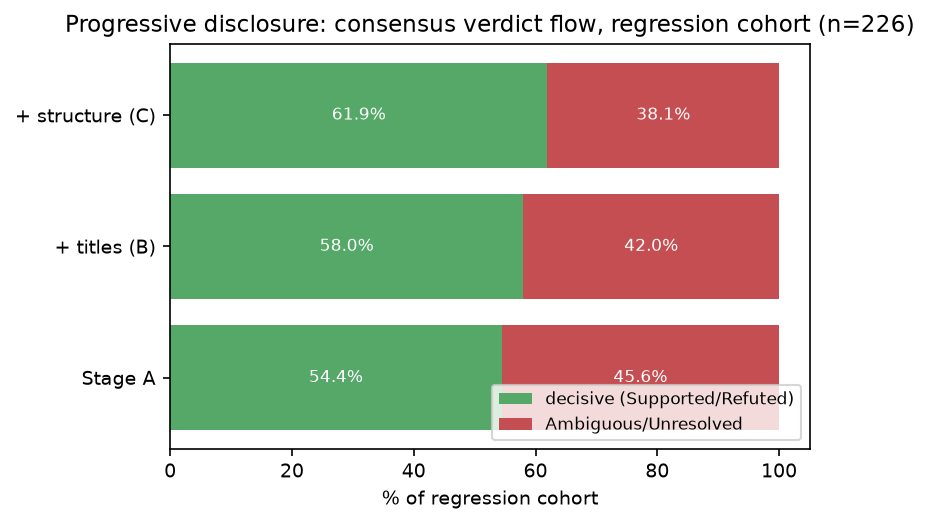
\includegraphics[width=0.85\linewidth]{../silver_adjudication_v1/cursor_panel/figures/fig3_resolution_flow.png}
\caption{Cursor/Grok resolution flow across Stages~A--C on the judged diagnostic cohort. Supplementary to Section~\ref{sec:rq3-grok}.}
\label{fig:flow}
\end{figure}

\begin{figure}[ht]
\centering
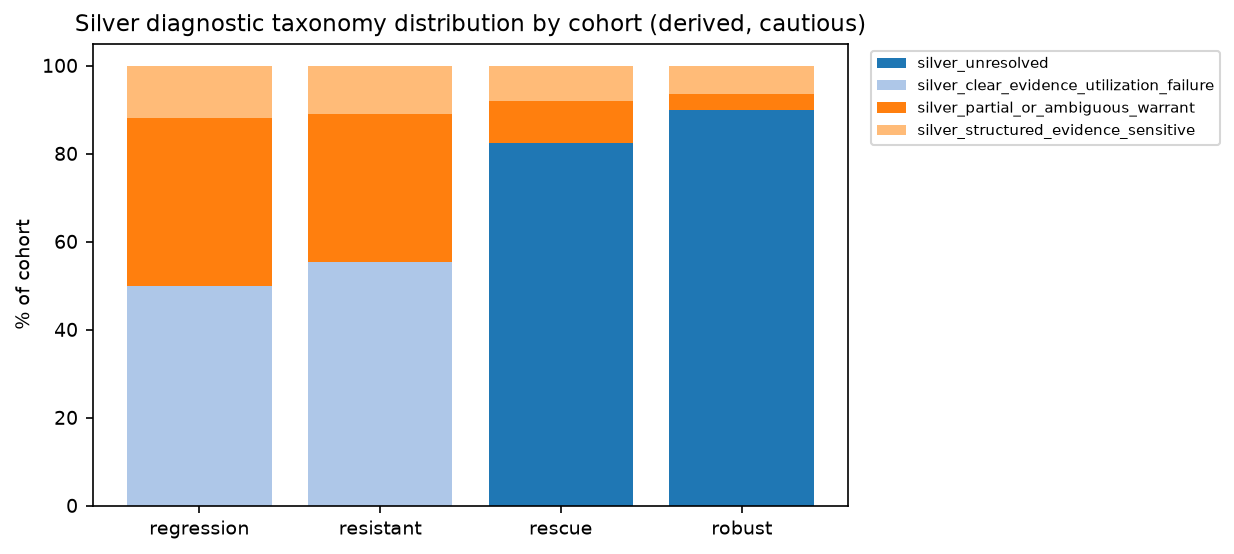
\includegraphics[width=0.75\linewidth]{../silver_adjudication_v1/cursor_panel/figures/fig7_taxonomy_distribution.png}
\caption{Cursor/Grok taxonomy distribution. Counts match Table~\ref{tab:mechanism-grok} on the 226 regressions.}
\label{fig:grok-tax}
\end{figure}

\begin{figure}[ht]
\centering
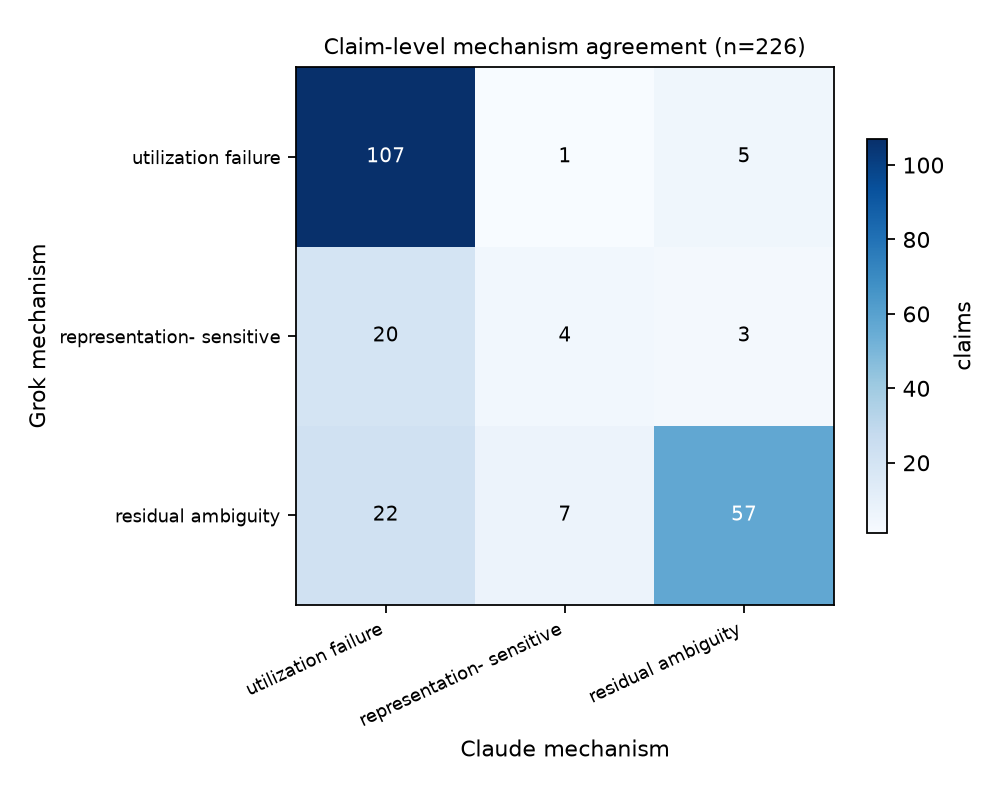
\includegraphics[width=0.88\linewidth]{../silver_adjudication_v1/claude_full_regression_panel/figures/fig3_mechanism_confusion.png}
\caption{Grok-versus-Claude taxonomy confusion on the 226 regressions. Disagreement is directional toward Claude utilization failure.}
\label{fig:confusion}
\end{figure}

\section{Denominator checklist}
\label{app:denoms}

\begin{tabular}{lr}
\toprule
Quantity & $n$ \\
\midrule
FEVER claims in the paired experiment & 10{,}000 \\
GPT predictions & 40{,}000 \\
Diagnostic-cohort claims constructed & 1{,}061 \\
Judged diagnostic-cohort items & 1{,}060 \\
Unique regressions & 226 \\
Grok Stage~C residual leftovers & 231 \\
Claude residual judgments & 1{,}155 \\
Claude full judgments & 3{,}390 \\
\bottomrule
\end{tabular}
